\documentclass[11pt,a4paper]{article}

% ---------- Packages ----------
\usepackage[utf8]{inputenc}
\usepackage[T1]{fontenc}
\usepackage[margin=2.3cm]{geometry}
\usepackage{lmodern}
\usepackage{microtype}
\usepackage{xcolor}
\usepackage{graphicx}
\usepackage{float}
\usepackage{enumitem}
\usepackage{titlesec}
\usepackage{listings}
\usepackage{tcolorbox}
\usepackage{amssymb}
\usepackage{booktabs}
\usepackage[hidelinks]{hyperref}
\usepackage{tikz}
\usetikzlibrary{arrows.meta,positioning,shapes.geometric,calc}

% ---------- Colors ----------
\definecolor{accent}{HTML}{1F6FB2}
\definecolor{accent2}{HTML}{0E7C5A}
\definecolor{codebg}{HTML}{F6F8FA}
\definecolor{codekw}{HTML}{A626A4}
\definecolor{codestr}{HTML}{50A14F}
\definecolor{codecom}{HTML}{8A8A8A}
\definecolor{boxbg}{HTML}{EFF5FB}

% ---------- Section styling ----------
\titleformat{\section}{\Large\bfseries\color{accent}}{\thesection}{0.6em}{}
\titleformat{\subsection}{\large\bfseries\color{accent2}}{\thesubsection}{0.6em}{}
\titlespacing*{\section}{0pt}{1.4ex plus 1ex minus .2ex}{1ex}

% ---------- Listings ----------
\lstdefinestyle{js}{
  backgroundcolor=\color{codebg},
  basicstyle=\ttfamily\scriptsize,
  keywordstyle=\color{codekw}\bfseries,
  stringstyle=\color{codestr},
  commentstyle=\color{codecom}\itshape,
  numberstyle=\tiny\color{codecom},
  showstringspaces=false,
  breaklines=true,
  frame=single,
  rulecolor=\color{codebg!60!gray},
  framesep=5pt,
  xleftmargin=6pt,
  language=Java,
  morekeywords={const,let,async,await,function,return,import,from,export,new,if,for,of,null,true,false},
  keepspaces=true,
  columns=fullflexible,
}
\lstset{style=js}

% ---------- Callout box ----------
\newtcolorbox{keybox}[1][]{colback=boxbg,colframe=accent,boxrule=0.8pt,
  arc=2pt,left=8pt,right=8pt,top=6pt,bottom=6pt,fonttitle=\bfseries\color{white},
  coltitle=white,colbacktitle=accent,title=#1}

\setlist{itemsep=2pt,topsep=3pt,parsep=0pt}

% ---------- Title ----------
\title{\vspace{-1.2cm}\textbf{\color{accent}Integrating the LLM Agent}\\[2pt]
\large Part 2 of the Autonomous Software Agents project --- a concrete plan grounded in \texttt{lab8-LLMs}}
\author{Autonomous Software Agents 2025--2026 \,\textbar\, University of Trento}
\date{June 2026}

\begin{document}
\maketitle
\vspace{-0.7cm}

% ============================================================
\section{Why this document}
Part 1 of the project delivered a working \textbf{BDI agent} (beliefs, deliberation, an
order-sensitive plan library, A\textsuperscript{*} movement and a PDDL crate-pushing detour).
Part 2 asks for an \textbf{LLM-based agent} that takes high-level objectives in natural
language, reasons over a memory of observations and a tool catalogue, produces a plan of
\emph{tool invocations}, and \textbf{cooperates with the BDI agent}. This note distils the
official \texttt{lab8-LLMs} reference code into a recipe for our codebase: the theory behind
each piece, and the concrete shape the JavaScript should take.

% ============================================================
\section{What lab8 actually teaches}
The lab is a 9-step ladder of \texttt{.mjs} files. Stripped of the toy examples, three design
decisions matter for us:

\begin{enumerate}
  \item \textbf{The LLM is reached through an OpenAI-compatible endpoint} (the faculty
  LiteLLM proxy). The same \texttt{openai} client library and message format work unchanged.
  \item \textbf{Tools are plain functions} collected in a dictionary. The model never touches
  the game; it \emph{names} a tool and the runtime executes it. This is exactly the indirection
  we need so the LLM can drive the Deliveroo SDK safely.
  \item \textbf{Reasoning is a text protocol}, not native function-calling. The lab uses the
  \textbf{ReAct} format (\texttt{Thought / Action / Action Input / Observation}) parsed with
  regexes, and a \textbf{Planner\,$\rightarrow$\,Executor} split for multi-step tasks.
\end{enumerate}

\begin{keybox}[Endpoint configuration (identical across every lab file)]
\begin{lstlisting}
import OpenAI from "openai";
const client = new OpenAI({
  baseURL: process.env.LITELLM_BASE_URL,   // https://llm.bears.disi.unitn.it/v1
  apiKey:  process.env.LITELLM_API_KEY,     // your faculty token
});
const MODEL = process.env.LOCAL_MODEL || "llama-3.3-70b-lmstudio";

async function callModel(messages, { temperature = 0 } = {}) {
  const r = await client.chat.completions.create({ model: MODEL, messages, temperature });
  return r.choices?.[0]?.message?.content ?? "";
}
\end{lstlisting}
\end{keybox}

\noindent Note: although the lab \emph{mentions} OpenAI native \texttt{tools}/\texttt{tool\_calls},
every solution file (including the Deliveroo one) actually uses the \textbf{manual text
protocol}. It is model-agnostic and works with the locally-hosted Llama model, so we adopt it too.

% ============================================================
\section{The theory in one page}

\begin{description}[leftmargin=1.4em,style=nextline]
  \item[Chain-of-Thought (CoT).] Ask the model to write its reasoning before its answer.
  In the lab this is the literal \texttt{Thought:} line. It improves multi-step decisions at
  the cost of tokens.
  \item[ReAct (Reason + Act).] Interleave reasoning with actions:
  \texttt{Thought $\to$ Action $\to$ Observation $\to$ Thought $\to \dots$}. The model emits
  \emph{one} action, the runtime executes it, feeds back an \texttt{Observation}, and loops.
  This is the backbone of the lab's execution loop and the natural fit for a partially
  observable game where each move reveals new tiles.
  \item[Planner / Executor.] For requests that need several steps, a \emph{planner} prompt
  first decomposes the objective into a short JSON list of steps; an \emph{executor} prompt then
  runs each step with its own ReAct mini-loop. This separates ``what to do'' from ``how to do
  it'' and keeps each prompt small.
  \item[Reflexion / Replanning.] When an action fails (a blocked tile, an expired parcel),
  the failure observation is fed back so the model revises its plan rather than repeating the
  mistake. Our BDI side already does this structurally (intention revision); on the LLM side it
  is a prompt-level feedback loop.
\end{description}

% ============================================================
\section{Reference architecture}

\begin{figure}[H]
\centering
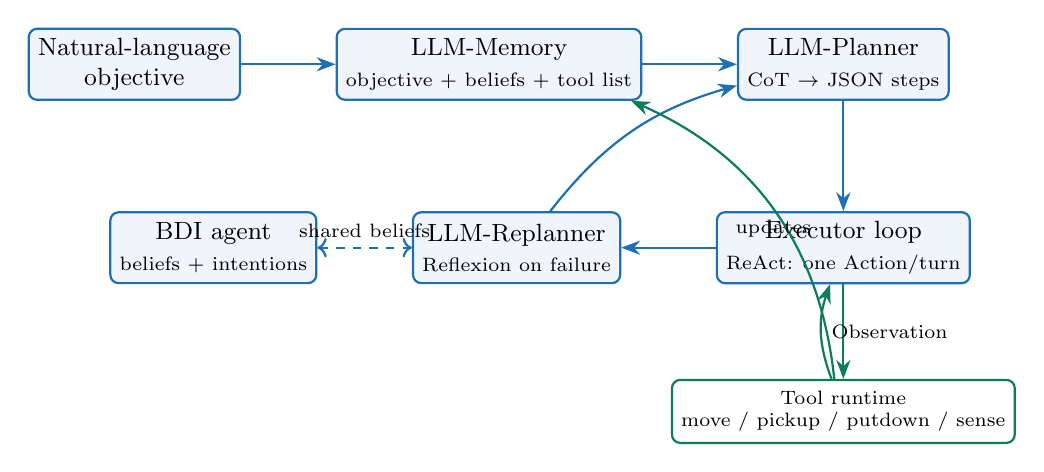
\begin{tikzpicture}[
  node distance=8mm and 12mm,
  box/.style={draw,rounded corners=3pt,align=center,minimum height=9mm,font=\small,fill=boxbg,draw=accent,thick},
  toolbox/.style={draw,rounded corners=3pt,align=center,minimum height=8mm,font=\scriptsize,fill=white,draw=accent2,thick},
  arr/.style={-{Stealth[length=2.4mm]},thick,draw=accent},
  arr2/.style={-{Stealth[length=2.4mm]},thick,draw=accent2},
]
\node[box] (obj) {Natural-language\\objective};
\node[box,right=of obj] (mem) {LLM-Memory\\\scriptsize objective + beliefs + tool list};
\node[box,right=of mem] (plan) {LLM-Planner\\\scriptsize CoT $\rightarrow$ JSON steps};
\node[box,below=14mm of plan] (exec) {Executor loop\\\scriptsize ReAct: one Action/turn};
\node[box,left=of exec] (replan) {LLM-Replanner\\\scriptsize Reflexion on failure};
\node[toolbox,below=12mm of exec] (tools) {Tool runtime\\\scriptsize move / pickup / putdown / sense};
\node[box,left=of replan] (bdi) {BDI agent\\\scriptsize beliefs + intentions};

\draw[arr] (obj) -- (mem);
\draw[arr] (mem) -- (plan);
\draw[arr] (plan) -- (exec);
\draw[arr] (exec) -- (replan);
\draw[arr] (replan) to[bend left=18] (plan);
\draw[arr2] (exec) -- (tools);
\draw[arr2] (tools) to[bend left=20] node[right,font=\scriptsize]{Observation} (exec);
\draw[arr,<->,dashed] (bdi) -- node[above,font=\scriptsize]{shared beliefs} (replan);
\draw[arr2] (tools) to[bend right=30] node[below,font=\scriptsize]{updates} (mem);
\end{tikzpicture}
\caption{The LLM agent loop. Boxes in blue are LLM-driven prompts; green is deterministic
runtime. The dashed link is the multi-agent channel to our existing BDI agent.}
\end{figure}

\noindent This maps cleanly onto the three components the project brief requires:
\textbf{LLM-Memory}, \textbf{LLM-Planner} (CoT), and \textbf{LLM-Replanner} (ReAct/Reflexion).

% ============================================================
\section{Concrete implementation for our codebase}

\subsection{1.\ Wrap the Deliveroo SDK as tools}
The lab's Deliveroo file exposes four tools; the agent only ever calls these. We extend the
set to the full action vocabulary from \texttt{docs/Context.md} \S3.1. Crucially, tools return
a \emph{string observation} --- including failures --- so the ReAct loop can react.

\begin{lstlisting}
import { DjsConnect } from "@unitn-asa/deliveroo-js-sdk/client";
const socket = DjsConnect(process.env.HOST, process.env.TOKEN);

const me = { id: null, x: null, y: null, score: 0 };
socket.onYou(you => Object.assign(me, you));

// Live beliefs the LLM can read (kept tiny on purpose)
const parcels = new Map();              // id -> {x,y,reward,carriedBy}
socket.onParcelsSensing(ps => { for (const p of ps) parcels.set(p.id, p); });

async function move(direction) {
  const d = direction.trim().toLowerCase();
  if (!["up","down","left","right"].includes(d))
    return `Error: invalid direction '${direction}'.`;
  const res = await socket.emitMove(d);
  return res ? `Moved ${d}. New position: ${JSON.stringify(res)}.`
             : `Error: move ${d} blocked (tile occupied or wall).`;
}
async function pick_up()  { const n = await socket.emitPickup();  return `Picked up ${n?.length ?? 0} parcel(s).`; }
async function put_down() { const n = await socket.emitPutdown(); return `Put down ${n?.length ?? 0} parcel(s).`; }
async function get_my_position() { return JSON.stringify(me); }
async function sense_parcels() {
  const free = [...parcels.values()].filter(p => !p.carriedBy);
  return free.length ? JSON.stringify(free) : "No parcels currently in view.";
}

const TOOLS = { move, pick_up, put_down, get_my_position, sense_parcels };
\end{lstlisting}

\subsection{2.\ The ReAct executor loop}
This is the heart of the lab (file \texttt{07A}/\texttt{9\_07C}). The model emits exactly one
\texttt{Action}; we execute it, append an \texttt{Observation}, and iterate up to a cap.

\begin{lstlisting}
function extractAction(t) {
  const a = t.match(/^Action:\s*(.+)$/im);
  const i = t.match(/^Action Input:\s*(.+)$/im);
  return (a && i) ? { action: a[1].trim(), input: i[1].trim() } : null;
}
function extractFinal(t) { const m = t.match(/^Final Answer:\s*([\s\S]*)$/im); return m ? m[1].trim() : null; }

async function runLoop(messages, maxIters = 8) {
  for (let i = 0; i < maxIters; i++) {
    const out = await callModel(messages, { temperature: 0 });
    messages.push({ role: "assistant", content: out });

    const act = extractAction(out);
    if (act) {
      const fn = TOOLS[act.action];
      const obs = fn ? await fn(act.input)
                     : `Error: unknown tool '${act.action}'. Available: ${Object.keys(TOOLS).join(", ")}`;
      messages.push({ role: "user", content: `Observation: ${obs}` });
      continue;                       // ReAct: act, observe, think again
    }
    const done = extractFinal(out);
    if (done) return done;
    messages.push({ role: "user", content: "Observation: invalid format. Output one Action or one Final Answer." });
  }
  return "Stopped: iteration limit reached.";
}
\end{lstlisting}

\subsection{3.\ The system prompt: memory + tools + protocol}
The prompt \emph{is} the LLM-Memory: it fuses the natural-language objective, a live snapshot
of beliefs, the tool catalogue, and the strict output contract. Regenerate the belief snapshot
each turn so the model always reasons over current state.

\begin{lstlisting}
function systemPrompt() {
  return [
    "You control a Deliveroo delivery agent on an MxN grid.",
    "Goal: maximise score by picking up parcels and delivering them to delivery tiles.",
    "",
    "World state (refreshed each turn):",
    `- Me: ${JSON.stringify(me)}`,
    `- Parcels in view: ${[...parcels.values()].map(p=>`(${p.x},${p.y}) r=${p.reward}`).join(", ") || "none"}`,
    "",
    "Tools: move(up|down|left|right), pick_up(), put_down(), get_my_position(), sense_parcels().",
    "Movement: up y+1, down y-1, right x+1, left x-1; one tile per call; a blocked tile fails.",
    "",
    "Output EXACTLY one of:",
    "  Thought: <reasoning>",        // Chain-of-Thought
    "  Action: <tool>",
    "  Action Input: <arg or none>",
    "OR, when the objective is done:",
    "  Thought: <reasoning>",
    "  Final Answer: <summary>",
    "Never invent tool results. Never output two Actions at once.",
  ].join("\n");
}
\end{lstlisting}

\subsection{4.\ Planner for multi-step objectives (CoT)}
For objectives like \emph{``collect the two nearest parcels then deliver''} the lab first
plans, then executes. The planner returns strict JSON; a fallback covers malformed output.

\begin{lstlisting}
const PLANNER_PROMPT = `You decompose a Deliveroo objective into 1-10 concrete steps.
Return ONLY JSON: {"steps":["step 1","step 2"]}  No markdown, no prose.`;

async function createPlan(objective) {
  const raw = await callModel(
    [{ role:"system", content: PLANNER_PROMPT }, { role:"user", content: objective }]);
  try { const p = JSON.parse(raw.replace(/```json|```/g,"").trim());
        if (Array.isArray(p.steps) && p.steps.length) return p; } catch {}
  return { steps: [objective] };                        // graceful fallback
}
\end{lstlisting}

\subsection{5.\ Replanning / Reflexion}
The executor already feeds failures back as \texttt{Observation}s, which is lightweight
Reflexion. Strengthen it by detecting repeated failures and re-invoking the planner with the
failure log appended --- the trigger conditions the brief lists (clock advanced, obstacle,
objective overridden) become explicit replan calls:

\begin{lstlisting}
if (consecutiveBlocked >= 2) {
  const note = `Previous attempt failed: ${lastObservation}. Replan around the obstacle.`;
  plan = await createPlan(`${objective}\n\nConstraint: ${note}`);
}
\end{lstlisting}

% ============================================================
\section{Multi-agent coordination (BDI $\leftrightarrow$ LLM)}
The brief (\S4.2) requires the two agents to exchange beliefs and divide tasks. Two practical
channels, in increasing ambition:

\begin{itemize}
  \item \textbf{Shared belief object.} Run both agents in one process (we already spawn
  several via \texttt{multiple\_run.js}); export the BDI \texttt{parcels}/\texttt{me} beliefs
  and let the LLM's \texttt{sense\_parcels} tool read the \emph{union} of both agents' views ---
  this gives the LLM visibility over hidden map regions the BDI agent has seen.
  \item \textbf{SDK \texttt{say}/\texttt{shout} messaging.} Use the Deliveroo communication
  channel so the agents negotiate: when a parcel is discovered, each agent reports its distance
  and the closer one claims it. The LLM is well suited to phrasing/parsing these natural-language
  hand-offs, while the BDI agent contributes precise A\textsuperscript{*} distances.
\end{itemize}

\noindent A clean rule of thumb: \textbf{BDI for fast, deterministic execution; LLM for
high-level objective interpretation and coordination}. The LLM's \texttt{move}/\texttt{pick\_up}
tools can even delegate to the existing \texttt{astar.js} \texttt{navigateTo()} instead of single
steps, reusing Part 1 wholesale.

% ============================================================
\section{Suggested file layout}
Add an \texttt{llmAgent/} sibling to \texttt{myAgent/}, reusing context and beliefs:

\begin{lstlisting}
llmAgent/
  llmClient.js     // OpenAI/LiteLLM wrapper + callModel()
  tools.js         // TOOLS dict wrapping the SDK (and optionally astar.navigateTo)
  memory.js        // systemPrompt() = objective + live beliefs + tool catalogue
  planner.js       // createPlan() (CoT, strict JSON)
  executor.js      // runLoop() (ReAct), replan trigger (Reflexion)
  coordination.js  // belief sharing + say/shout negotiation with the BDI agent
  llmAgent.js      // entry: read NL objective -> plan -> execute -> report
.env               // LITELLM_BASE_URL, LITELLM_API_KEY, LOCAL_MODEL, HOST, TOKEN, NAME
\end{lstlisting}

\begin{keybox}[Minimal milestone order]
\textbf{(a)} endpoint + \texttt{callModel} \;$\to$\; \textbf{(b)} four SDK tools + ReAct loop
(reproduce lab \texttt{9\_07C}) \;$\to$\; \textbf{(c)} planner/executor split \;$\to$\;
\textbf{(d)} Reflexion replanning \;$\to$\; \textbf{(e)} BDI belief sharing + negotiation.
Each step is independently demonstrable.
\end{keybox}

\vspace{0.3cm}
\noindent\textit{Source: \texttt{unitn-ASA/DeliverooAgent.js/lab8-LLMs} (files \texttt{04}--\texttt{09},
notably \texttt{9\_07C\_DeliverooAgent.mjs} and
\texttt{09\_08B-planner-execution-loop\_DeliverooJS\_EXTRA.mjs}) and project \texttt{docs/Context.md}.}

\end{document}
